\documentclass[a4paper,11pt,fleqn]{article}%fleqn pour aligner les equations à gauche
\usepackage{../../Styles/Eval}


\newcommand{\chnum}{Chapitre 1 et 2}
\newcommand{\chtitle}{Transformation acide-base et pH}
\newcommand{\dtype}{DS 1}

\begin{document}
\maketitle

\section{Beurre acide}
\noindent \colorbox{red!10}{\begin{minipage}{.98\linewidth}
	\small
	\textbf{Acide butyrique}\\
	Les travaux de Crevreul lui ont permis d’isoler un acide gras à quatre atomes de carbone, qu’il a nommé « acide butyrique », dérivé du latin \textit{butyrum} signifiant « \textit{beurre} », à cause de son odeur caractéristique de beurre rance. Pour la suite, l’élément but(y)- a été repris pour former les noms de molécules à quatre atomes de carbone dont, avec le suffixe -ane des alcane, celui du butane.\\
\end{minipage}}

L’acide butyrique est un acide carboxylique possédant une chaîne carbonée, dérivée du butane. Il est présent dans le couple acide butyrique/ion butyrate (\ce{C4H8O2}/\ce{C4H7O2-}).
\begin{enumerate}
	\item Déterminer le schéma de Lewis de l’acide butyrique. (0,5pt)
	\item Justifier le caractère "acide" de la molécule. (1pt)
	\item Écrire la demi-équation associée à l'acide butyrique. (0,5pt)
	\item Écrire l'équation de la réaction mise en jeu lorsque l'acide butyrique est mis dans l'eau. (1pt)
	\item On réalise une solution d'acide butyrique à partir d'une masse de \SI{2,2}{\milli\gram} dissous dans \SI{500}{\milli\liter} d'eau. En partant de l'hypothèse que tout l'acide réagit avec l'eau, déterminer le pH de la solution obtenue. (1pt)
\end{enumerate}
Le butanoate de méthyle \ce{CH3(CH2)2COOCH3} est un composé chimique utilisé comme arôme pour son odeur de pomme. Il est obtenu à partir de l’acide butyrique.
\begin{enumerate}[resume]
	\item Recopier puis compléter le schéma de Lewis du butanoate de méthyle suivant, puis identifier les éventuels groupes fonctionnels. (0,5pt)
	\item Préciser si l’ester formé a un caractère acide. (0,5pt)
	\item Attribuer chacun des spectres suivants à la molécule (acide butyrique ou butanoate de méthyle) correspondante en justifiant. (1pt)
\end{enumerate}

\begin{figure}[h!]
	\centering \chemfig[atom sep = 2em]{CH_3-CH_2-CH_2-C(=[1]O)-[7]O-CH_3}
	\caption{Butanoate de méthyle}

	\begin{minipage}{.48\linewidth}
		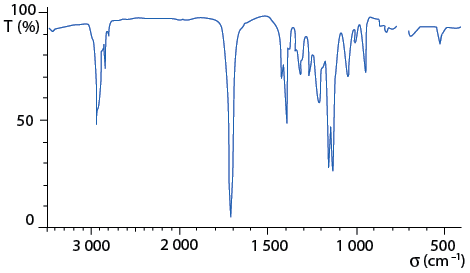
\includegraphics[width=.9\linewidth]{Ressources/Butanoate de méthyle1.png}
	\end{minipage}\hspace{.02\linewidth}
	\begin{minipage}{.48\linewidth}
		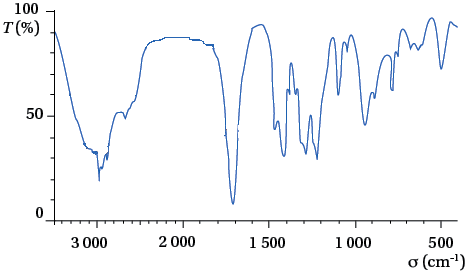
\includegraphics[width=.9\linewidth]{Ressources/Butanoic1.png}
	\end{minipage}
	\caption{Spectres IR à attribuer}
\end{figure}

\newpage
\section{Les ions nickel}
On dispose d'une solution $S_1$ de chlorure de nickel (\ce{Ni^{2+}(aq)} ; \ce{2Cl-(aq)}) de concentration $c_1$ en soluté apporté. on souhaite déterminer cette concentration de trois manières différentes :
\begin{itemize}
	\item en mesurant la conductivité de la solution : on trouve $\sigma$ = \SI{7,556}{\milli\siemens\per\centi\meter}
	\item en mesurant l'absorbance l'absorbance de la solution : on obtient $A$ = \SI{0,663}{} à $\lambda$ = \SI{720}{nm}
	\item en faisant réagir $V$ = \SI{10.0}{mL} de la solution avec $V$ = \SI{10.0}{mL} d'hydroxyde de sodium \ce{NaOH(aq)} de concentration $c_2$ = \SI{0,100}{\mole\per\liter}, il se forme de l'hydroxyde de nickel \ce{Ni(OH)2(s)} insoluble. On mesure alors la conductivité de la solution $\sigma_f$ = \SI{8,784}{\milli\siemens\per\centi\meter}.
\end{itemize}

\begin{enumerate}
	\item Déterminer la couleur apparente d'une solution de chlorure de nickel. (1pt)
	\item Déterminer la concentration en quantité de matière $c_1$ obtenue par la première méthode. (1pt)
	\item Déterminer la concentration en quantité de matière $c_1$ obtenue par la deuxième méthode. (1pt)
	\item Écrire l'équation de la réaction de précipitation entre les ions \ce{Ni^{2+}(aq)} et les ions hydroxyde \ce{HO-(aq)}. On fera apparaître, dans ce cas précis, les ions spectateurs, présents en solution. (1pt)
	\item Établir l'expression de la conductivité $\sigma_f$ en fonction des concentrations $c_1$ et $c_2$ et des conductivités molaires ioniques des ions présents à l'état final. (2pts)
	\item En déduire la valeur de la concentration $c_1$. (1pt)
\end{enumerate}

\begin{figure}[h!]
\centering
\begin{minipage}{.58\linewidth}
	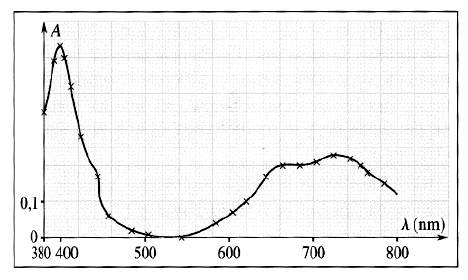
\includegraphics[width=\linewidth]{Ressources/TSPE_DS1_Fig1.png}
	\caption{Spectre d'absorbance du chlorure de nickel}
\end{minipage}\hspace{.02\linewidth}
\begin{minipage}{.38\linewidth}
	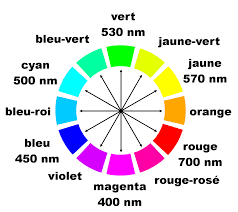
\includegraphics[width=\linewidth]{Ressources/TSPE_C2_Fig2.png}
	\caption{Cercle chromatique}
\end{minipage}
\end{figure}

\noindent \colorbox{yellow!10}{\begin{minipage}{.95\linewidth}
	\textbf{Données :}\\
	\begin{tabular}{m{8cm} |m{8.5cm}}
	\textbf{Conductivités molaires ioniques à \SI{25}{\celsius}, tenant compte du nombre de  charges : } & \textbf{Coefficient d'absorption molaire des ions nickel \ce{Ni^{2+}(aq)} à \SI{720}{nm} :}\\
	$\lambda$(\ce{Cl-}) = \SI{7,6}{\milli\siemens\meter\squared\per\mole} & $\epsilon$ = \SI{22,1}{\liter\per\mole\per\centi\meter}\\
	$\lambda$(\ce{Ni^{2+}}) = \SI{9,9}{\milli\siemens\meter\squared\per\mole} & \textbf{Longueur de la cuve de spectrophotométrie :} \\
	$\lambda$(\ce{HO-}) = \SI{19,8}{\milli\siemens\meter\squared\per\mole} & $l$ = \SI{1,0}{cm}\\
	$\lambda$(\ce{Na+}) = \SI{5,0}{\milli\siemens\meter\squared\per\mole} &\\
	\end{tabular}
	
\end{minipage}}

\end{document}